\chapter{Evaluation}

Zu Beginn der Arbeit wurde der Ansatz zur Erstellung des Umweltmodells verfolgt, welches allerdings in eine Sackgasse führte, durch den späten Paradigmenwechsel von Spatial Mapping zu \ac{SLAM} blieb wenig Zeit, den Ansatz zu verfeinern, er ist jedoch sehr vielversprechend und hat ein großes Potential.
Zudem war die Fehlerbehebung an der Drohne ziemlich zeitaufwändig, wodurch die Bearbeitung der anderen Bereiche zwischenzeitlich in den Hintergrund gerutscht sind.

\section{Analyse der Ergebnisse}
\subsection{Sensordrift Drohne}

Mit der Boardkamera + \ac{IMU} Daten konnte keine stabile Position gehalten werden. Die Aufgabe der Datenfusion hat in diesem Fall die PX4 Autopilot Software auf dem COEX Pix übernommen.
Durch den akkumulierten Fehler der \ac{IMU} Daten driftete die Drohne aber immer nach gewisser Zeit weg. In der Simulation hat die Konfiguration jedoch ohne Probleme funktioniert, da dort der akkumulierte Fehler nicht vorhanden ist.
Es ist anzumerken, dass die Simulation keine realen Bedingungen widerspiegelt und daher möglicherweise nicht alle Herausforderungen und Unsicherheiten, die in der realen Welt auftreten können, berücksichtigt. Daher ist es wichtig, die Evaluierungsergebnisse der Simulation mit Vorsicht zu interpretieren und die Realität in Betracht zu ziehen. Weitere Untersuchungen und Experimente sollten durchgeführt werden, um die Ursachen des akkumulierten Fehlers der \ac{IMU}-Daten zu identifizieren und geeignete Maßnahmen zur Fehlerkompensation zu entwickeln.


\subsection{Umsetzung SLAM auf Raspberry Pi}

\subsubsection{Kamerazugriff}

Die HoloLens 2 bietet im Vergleich zur Azure Kinect keinen direkten Echtzeitzugriff zur Verwendung von \ac{SLAM}. Bei der HoloLens 2 muss man sich darauf verlassen, dass die HoloLens 2 das Modell der Umgebung schnell genug aktualisiert. Da wir wie in Kapitel \ref{mechanische-herausforderungen:section} beschrieben die HoloLens 2 nicht auf der Drohne montieren können, resultiert dies darin, dass wir vor dem Flug die Umgebung in ein 3D Modell überführen müssen. Deshalb kann jedoch auch die Spatial Mapping Funktion der HoloLens nicht verwendet werden, da diese nur funktioniert, wenn die HoloLens 2 beim Flug dabei ist.
Die Spatial Mapping Funktion funktioniert nicht, da die Positionierung von der Position der Sensoren der HoloLens 2 abhängt.
Durch den direkten Kamerazugriff der Azure Kinect kann \ac{VSLAM} direkt mit den Rohdaten dieser durchgeführt werden. Da die Kinect auf der Drohne montiert werden kann, wird direkt eine Karte der Umgebung erstellt und die Lokalisierung der Drohne beziehungsweise der Kamera durchgeführt. Es muss also kein Vorabscan der Umgebung mehr durchgeführt werden. Der \ac{VSLAM} Ansatz ist allerdings sehr rechenaufwendig, aber für Einsätze mit Drohnen in Gebäuden notwendig, um Hindernisse frühzeitig zu erkennen. Da die Drohne auch in unbekannten Umgebungen eingesetzt werden soll, ist es keine Option vor dem Flug der Drohne einen 3D-Scan der Umgebung durchzuführen. Wenn schon die Position in einem 3D Modell durch visuelle Analysen bestimmt werden muss, kann auch gleich \ac{SLAM} eingesetzt werden.

\subsubsection{Kartenerstellung \& Odometrie}

Die Evaluierung der Kartengenerierung und Odometrie in Visual SLAM-basierten Systemen auf Drohnen zeigt vielversprechende Ergebnisse in Bezug hinsichtlich von Genauigkeit und Zuverlässigkeit der generierten Karten sowie der geschätzten Odometrieinformationen. Für diese Aufgabe wurde eine Azure Kinect verwendet, um sowohl visuelle als auch Tiefeninformationen zu erfassen. Darüber hinaus wurden \ac{IMU}-Daten zur Verbesserung der Trajektorie verwendet.

Die Ergebnisse zeigen, dass die Kombination aus RGB-Bildern und Tiefeninformationen der Azure Kinect eine genauere und detailliertere Kartierung ermöglicht. Die Tiefeninformationen helfen dabei, die räumliche Struktur besser zu erfassen und die Genauigkeit der erstellten Karten zu verbessern. Durch die Verschmelzung der visuellen und der Tiefeninformationen kann die Drohne zuverlässig navigieren und selbst in Umgebungen mit geringer Textur oder gleichmäßigen Oberflächen genaue Karten erstellen.

Die Integration von \ac{IMU}-Daten ermöglicht eine verbesserte Odometrieschätzung und eine robustere Trajektorienberechnung. Zudem verringert die Kombination von visuellen Daten, Tiefeninformationen und IMU-Daten den Drift der geschätzten Flugbahn. Die \ac{IMU}-Daten liefern wichtige Informationen über die Beschleunigung und Ausrichtung der Drohne, was zu einer genaueren Schätzung der aktuellen Position und Ausrichtung führt.

Dennoch wurden bei der Bewertung einige Probleme festgestellt. In bestimmten Situationen, z.B. bei schnellen Bewegungen oder starken Vibrationen, konnten die \ac{IMU}-Daten Rauschen aufweisen, was zu einer geringeren Genauigkeit der Flugbahn führte. Es wurden jedoch Filter- und Fusionstechniken angewandt, um das Rauschen zu reduzieren und eine robuste Flugbahnberechnung zu gewährleisten.

Um die Leistung der Kartenerstellung und Odometrie weiter zu verbessern, könnten zusätzliche Optimierungen und Anpassungen vorgenommen werden. Dazu gehören die Verfeinerung der Fusionstechniken von Sicht-, Tiefen- und IMU-Daten sowie die Integration weiterer Sensorinformationen. Außerdem könnten fortgeschrittene Algorithmen zur Trajektorienoptimierung und Rauschfilterung eingesetzt werden.

Insgesamt zeigt die Auswertung, dass die Verwendung von Azure Kinect in Kombination mit \ac{IMU}-Daten eine effektive Methode zur Verbesserung der Kartenerstellung und Odometrie in Visual SLAM-basierten Systemen auf Drohnen ist. Durch die Integration von RGBD-Tiefenkamera- und \ac{IMU}-Daten konnten die Genauigkeit, Robustheit sowie Zuverlässigkeit der geschätzten Flugbahn erhöht werden, was zu präzisen und zuverlässigen autonomen Flugmanövern führt.

Um die Leistung des \ac{SLAM} Algorithmus mit der Azure Kinect Kamera zu beurteilen, haben wir auch den ORB-SLAM3 Algorithmus mit Testdaten laufen lassen. Genauer gesagt mit dem Testdatensatz Floor1 von der \ac{TUM} von \cite{tum_data}.

Ein Beispiel davon sehen sie in Abbildung \ref{fig:orbslam3}

\begin{figure}
    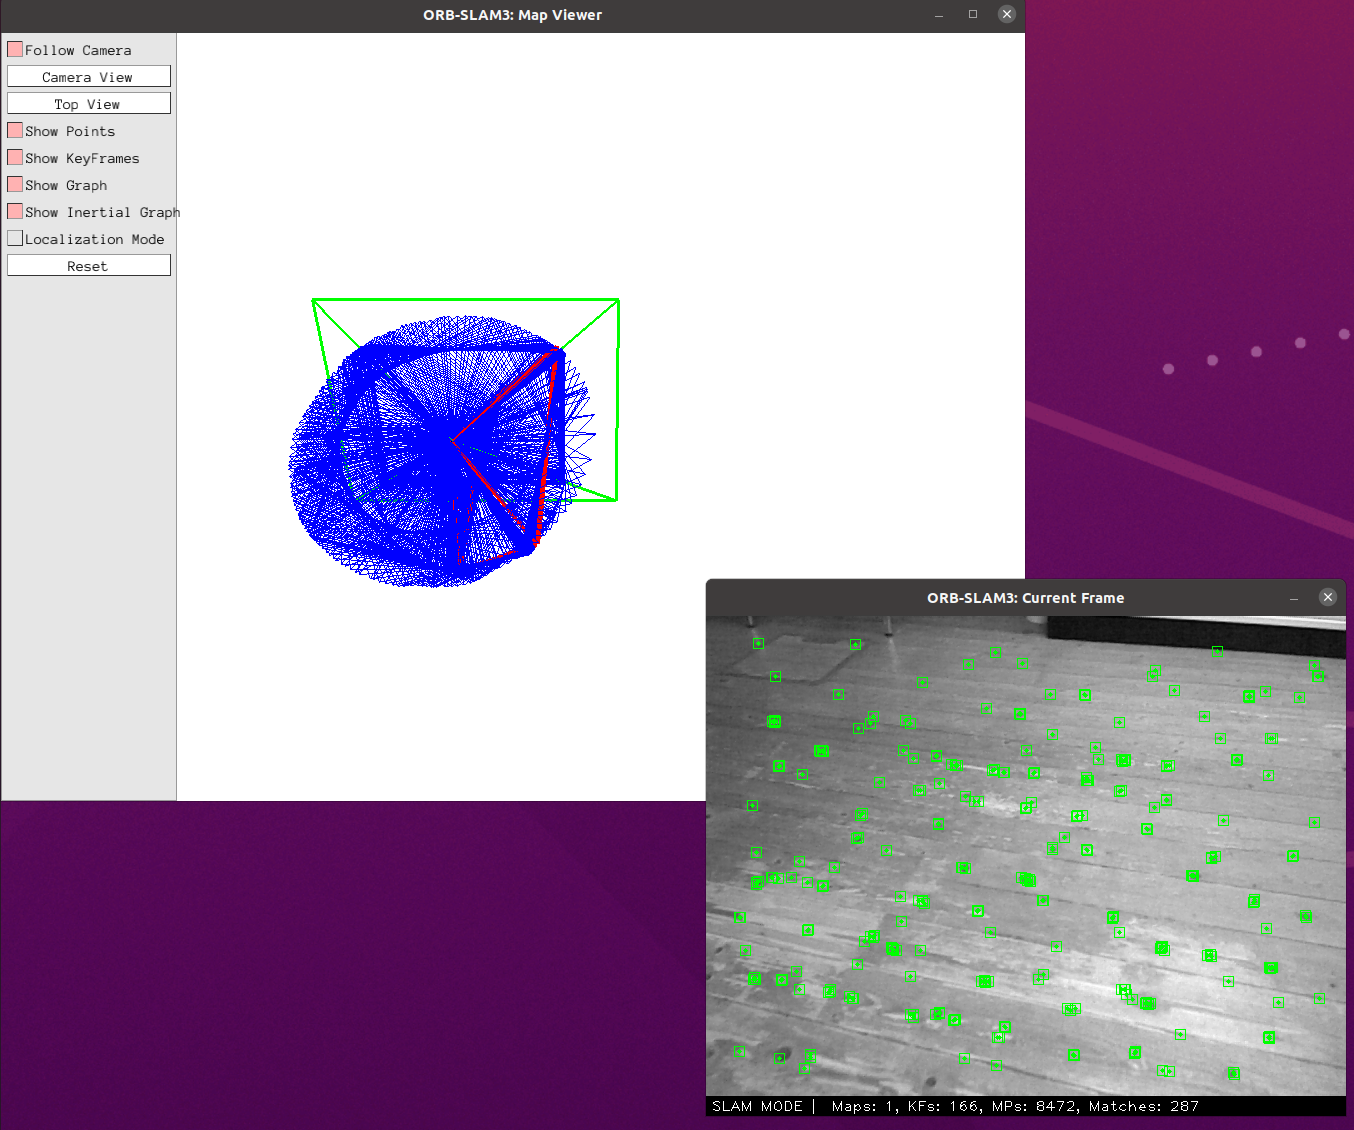
\includegraphics[width=\textwidth]{images/orbslam3_simulation}
    \label{fig:orbslam3}
    \caption{ORB-SLAM3 Simulation}
\end{figure}

\subsection{Trajektorenbestimmung}
Die Auswertung der Trajektorienbestimmung mit \ac{VSLAM} zeigt vielversprechende Ergebnisse für eine genaue und robuste Positionsbestimmung. \ac{VSLAM} ermöglicht hierbei die gleichzeitige Schätzung der Kameraposition und die Erstellung einer 3D-Karte der Umgebung auf Grundlage visueller Merkmale. Bei der Analyse verschiedener Parameter und Einstellungen zur Optimierung der Genauigkeit und Zuverlässigkeit der Trajektorienbestimmung zeigte sich, dass \ac{VSLAM} in der Lage ist, die Kameraposition mit hoher Genauigkeit und Stabilität auch in Umgebungen mit wechselnden Lichtverhältnissen und unterschiedlichen Texturen zu bestimmen. Insgesamt war die Trajektorienbestimmung konsistent und folgte den Kamerabewegungen mit geringen Abweichungen. Dennoch wurden einige Probleme festgestellt, wie beispielsweise das Auftreten von Drift oder Verlust der Verfolgung. Diese Probleme können auf die begrenzte Rechenleistung des verwendeten Raspberry Pi sowie die Komplexität der verwendeten Algorithmen zurückgeführt werden. Insgesamt ist die Trajektorienbestimmung mit \ac{VSLAM} eine vielversprechende Methode, um eine präzise und robuste Positionsbestimmung in Echtzeit zu ermöglichen. Dennoch sind weitere Optimierungen und Anpassungen erforderlich, um die Leistung in anspruchsvolleren Szenarien weiter zu verbessern.
\subsubsection{Pfadfindung/Navigation}

Die Bewertung der Wegfindung und Navigation in visuellen SLAM-basierten Systemen für Drohnen zeigt vielversprechende Ergebnisse bei autonomen Drohnenflügen. Durch die Erstellung eines Umweltmodells in Echtzeit ist es mit visuellem SLAM möglich, effektive Flugwege zu planen und Hindernissen auszuweichen. Bei Tests zur Bahngenauigkeit, der Kollisionsvermeidung und der Zuverlässigkeit des Navigationssystems zeigte sich, dass die Drohnen nun in der Lage waren, genaue Pfade zu berechnen und Hindernissen erfolgreich auszuweichen. Jedoch ergibt sich auch hier wieder das Problem, dass die Leistung des Raspberry Pi nicht ausreicht, da dieser bereits für bei der Erstellung des Umweltmodells Probleme bereitete. In der Simulation konnte hingegen eine funktionierende Lokalisierung und Navigation umgesetzt werden, da in der Simulation die Leistung nicht durch den Raspberry PI beschränkt war.

\subsubsection{Berechnungsressourcen}

\ac{VSLAM} umfasst komplexe Algorithmen zur Erkennung und Verfolgung visueller Merkmale in Echtzeit, zur Schätzung der Kameraposition und zur Erstellung einer Karte der Umgebung. Diese Algorithmen erfordern eine große Anzahl von Berechnungen, einschließlich Bildverarbeitung, Merkmalsextraktion, Merkmalsverfolgung, Kamerakalibrierung und Optimierung. Obwohl der Raspberry Pi über eine leistungsfähige CPU und eine spezielle Grafikeinheit verfügt, sind seine Ressourcen wie Rechenleistung, Speicher und Bandbreite im Vergleich zu Desktop-Computern oder Hochleistungsprozessoren begrenzt. Diese begrenzten Ressourcen können die Echtzeitleistung und Genauigkeit von \ac{VSLAM} beeinträchtigen. Die Einschränkungen des Raspberry Pi machen es daher schwierig, \ac{VSLAM} in anspruchsvollen Anwendungen einzusetzen, die eine kontinuierliche Echtzeitverarbeitung und hohe Genauigkeit erfordern.

\subsection{Steuerung der Drohne mittels ROS}\label{steuerung_drohne_ros:subsection}
Die Steuerung mittels \ac{ROS} bietet vielzählige Möglichkeiten die Steuerung der Drohne zu optimieren. Durch dieses System wird es ermöglicht eigene Skripte zu testen, aber auch Datenströme der Kamera oder auch andere externe Sensoren und Systeme zu benutzen, um beispielsweise Algorithmen zur Erstellung von Umweltmodellen wie \ac{SLAM} auf dem Raspberry Pi zu ermöglichen. Zudem ist \ac{ROS} hierbei sehr flexibel und bietet dabei jede Menge Dokumentationen.
Allerdings gab es auch Probleme, besonders mit der Verwendung von ROS2, da hierbei einige Pakete noch nicht auf das neuere System angepasst waren und so eine Vielzahl an Schwierigkeiten mit sich gebracht haben. Durch die Vielzahl an \ac{ROS} Versionen die es gibt, die auch alle unterschiedliche Funktionalitäten und Kompatibilitäten aufweisen, kommt es oft zu Situationen in denen zwei verschiedene Pakete nicht für die jeweilige \ac{ROS} Version verfügbar bzw. kompatibel sind.


\subsection{Mechanische Herausforderungen}\label{mechanische-herausforderungen:section}

Da der erste Ansatz beinhaltete die HoloLens 2 auf der Drohne zu montieren, mussten schon frühzeitig Überlegungen evaluiert werden, welche die Befestigung der HoloLens 2 an der COEX Drohne ermöglichen. Schnell wurde jedoch ersichtlich, dass die Drohne nicht für diese Art von Nutzlast geeignet ist. Die HoloLens ist zu groß und vor allem zu schwer und übersteigt dadurch auch das offizielle Maximalgewicht der Coex Clover Drohne. Desweiteren würde die Montage der HoloLens die Flugdauer der Drohne stark reduzieren, da mehr Energie benötigt wird. Zudem wird die Steuerung und Regelung der Drohne durch das wesentlich höhere Gewicht unnötig stark erschwert. Außerdem sind die Kosten der HoloLens 2 in keinem Verhältnis zu den Risiken einer Beschädigung, die durch eine Fehlfunktionalität der COEX Drohne ausgelöst wird. Die HoloLens 2 bietet auch keine Montagemöglichkeiten auf der Drohne, da sie nicht für diesen Einsatzzweck konzipiert wurde. Bei der HoloLens 2 handelt es sich um eine \ac{AR} Brille und nicht um eine mobile Kamera für Robotik Anwendungen.

Im Gegensatz dazu besitzt die Azure Kinect die gleiche Kamerahardware wie die HoloLens 2, wurde jedoch für solche Anwendungen konzipiert. Sie ist deutlich kleiner und platzsparender und bietet Montagemöglichkeiten an der COEX Drohne. 

\section{Interpretation der Ergebnisse}

Die Auswertung der verwendeten Sensoren und Algorithmen zeigt, dass die Verwendung der Azure Kinect in Kombination mit \ac{IMU}-Daten vielversprechende Ergebnisse für die Kartierung, Odometrie, Trajektorienbestimmung und Navigation auf einer Drohne liefert. Die Kombination dieser Datenquellen verringert den Drift und verbessert die Genauigkeit der geschätzten Flugbahn.

Dennoch gibt es einige Probleme, die zu beachten sind. Diese sind zum einen die begrenzte Verarbeitungsleistung des Raspberry Pi, was zu Einschränkungen und Verzögerungen bei der Echtzeitverarbeitung der visuellen Daten führt. Dies kann die Reaktionsfähigkeit und Stabilität des Navigationssystems beeinträchtigen. Daher sollten weitere Optimierungen und die Verwendung leistungsfähigerer Hardware in Betracht gezogen werden, um \ac{VSLAM} mit der Pfadfindung auf der Drohne optimal einsetzen zu können.

Die mechanischen Herausforderungen, die mit der Montage der Sensoren an der Drohne verbunden sind, wurden ebenfalls festgestellt. Die HoloLens 2 erweist sich aufgrund ihrer Größe, ihres Gewichts und fehlender Befestigungsmöglichkeiten als ungeeignet. Die Azure Kinect hingegen ist kleiner, leichter und bietet Befestigungsmöglichkeiten für den Einsatz an der Drohne.

\subsection{Schlussfolgerung}
Zusammenfassend kann festgehalten werden, dass die Verwendung von RGBD-Tiefenkameras wie die Azure Kinect in Kombination mit \ac{IMU}-Daten eine vielversprechende Lösung für die autonome Navigation von Drohnen in Innenräumen darstellt. Durch die Kombination von visuellen Daten, Tiefeninformationen und \ac{IMU}-Daten können präzise Karten der Umgebung erstellt, genaue Trajektorien geschätzt und zuverlässige autonome Flugmanöver durchgeführt werden. Um die volle Leistungsfähigkeit und Robustheit des Systems zu erreichen, müssen jedoch einige Probleme wie die fehlende Rechenleistung oder auch der Sensordrift der Coex Drohne behoben werden. \\
Dennoch wurden wichtige Erkenntnisse für den autonomen Flug von Drohnen in Gebäuden ohne die Verwendung von \ac{GPS} gesammelt.



